\documentclass[tikz]{standalone}\usepackage[]{graphicx}\usepackage[]{xcolor}
% maxwidth is the original width if it is less than linewidth
% otherwise use linewidth (to make sure the graphics do not exceed the margin)
\makeatletter
\def\maxwidth{ %
  \ifdim\Gin@nat@width>\linewidth
    \linewidth
  \else
    \Gin@nat@width
  \fi
}
\makeatother

\definecolor{fgcolor}{rgb}{0.345, 0.345, 0.345}
\newcommand{\hlnum}[1]{\textcolor[rgb]{0.686,0.059,0.569}{#1}}%
\newcommand{\hlsng}[1]{\textcolor[rgb]{0.192,0.494,0.8}{#1}}%
\newcommand{\hlcom}[1]{\textcolor[rgb]{0.678,0.584,0.686}{\textit{#1}}}%
\newcommand{\hlopt}[1]{\textcolor[rgb]{0,0,0}{#1}}%
\newcommand{\hldef}[1]{\textcolor[rgb]{0.345,0.345,0.345}{#1}}%
\newcommand{\hlkwa}[1]{\textcolor[rgb]{0.161,0.373,0.58}{\textbf{#1}}}%
\newcommand{\hlkwb}[1]{\textcolor[rgb]{0.69,0.353,0.396}{#1}}%
\newcommand{\hlkwc}[1]{\textcolor[rgb]{0.333,0.667,0.333}{#1}}%
\newcommand{\hlkwd}[1]{\textcolor[rgb]{0.737,0.353,0.396}{\textbf{#1}}}%
\let\hlipl\hlkwb

\usepackage{framed}
\makeatletter
\newenvironment{kframe}{%
 \def\at@end@of@kframe{}%
 \ifinner\ifhmode%
  \def\at@end@of@kframe{\end{minipage}}%
  \begin{minipage}{\columnwidth}%
 \fi\fi%
 \def\FrameCommand##1{\hskip\@totalleftmargin \hskip-\fboxsep
 \colorbox{shadecolor}{##1}\hskip-\fboxsep
     % There is no \\@totalrightmargin, so:
     \hskip-\linewidth \hskip-\@totalleftmargin \hskip\columnwidth}%
 \MakeFramed {\advance\hsize-\width
   \@totalleftmargin\z@ \linewidth\hsize
   \@setminipage}}%
 {\par\unskip\endMakeFramed%
 \at@end@of@kframe}
\makeatother

\definecolor{shadecolor}{rgb}{.97, .97, .97}
\definecolor{messagecolor}{rgb}{0, 0, 0}
\definecolor{warningcolor}{rgb}{1, 0, 1}
\definecolor{errorcolor}{rgb}{1, 0, 0}
\newenvironment{knitrout}{}{} % an empty environment to be redefined in TeX

\usepackage{alltt}
\usepackage{tikz}
\usepackage{amsmath,amsthm,amssymb}
\usepackage{mathrsfs}
\usetikzlibrary{arrows.meta}
\IfFileExists{upquote.sty}{\usepackage{upquote}}{}
\begin{document}

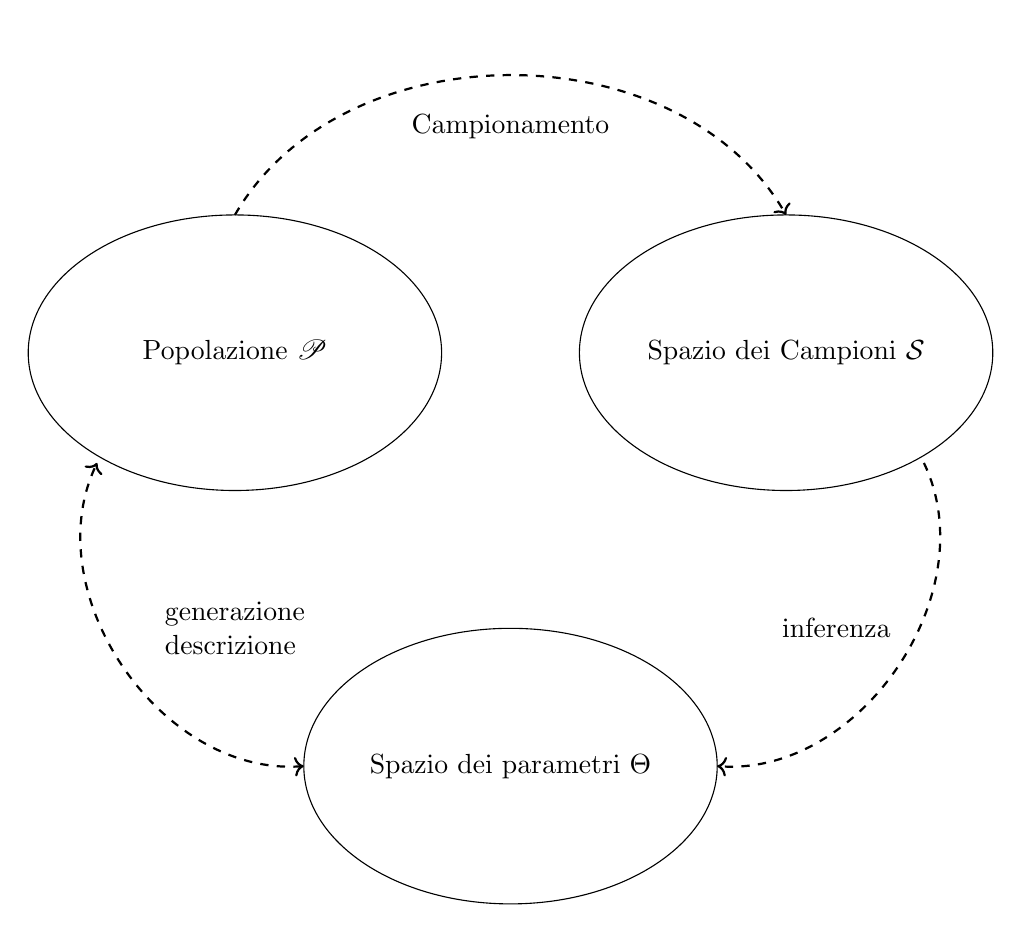
\begin{tikzpicture}[scale=3.5]

% Ellissi
\draw    (-1,1) ellipse (.75 and 0.5);
\draw   ( 1,1) ellipse (.75 and 0.5);
\draw     ( 0,-.5) ellipse (.75 and 0.5);

% Testo nei tre ovali
\node at (-1,1)    {Popolazione  $\mathscr{P}$};
\node at ( 1,1)    {Spazio dei Campioni $\mathcal{S}$};
\node at ( 0,-.5) {Spazio dei parametri $\Theta$};

% Freccia osservazione
\draw[->, thick, dashed] (-1 ,1.5) to [bend left=60] (1 ,1.5);
\node[below] at (0,1.9) {Campionamento};

% Freccia inferenza (campione -> modello)
\draw[->, thick, dashed] (1.5 ,0.6) to [bend left=60] (0.75,-0.5);
\node[align=left, right] at (0.95,0) {inferenza};

% Freccia simulazione (modello -> popolazione)
\draw[<->, thick, dashed] (-0.75,-0.5) to [bend left=60] (-1.5 ,0.6);
\node[align=left] at (-1,0) {generazione\\descrizione};


\end{tikzpicture}

% 
% 
% \begin{tikzpicture}[scale=3.5]
% 
% % Ellissi
% \draw    (-1,1) ellipse (.75 and 0.5);
% \draw   ( 1,1) ellipse (.75 and 0.5);
% \draw     ( 0,-.5) ellipse (.75 and 0.5);
% 
% % Testo nei tre ovali
% \node at (-1.3,1.5)    {$\mathscr{P}$};
% \node at ( 1.3,1.5)    {$\mathcal{S}$};
% \node at ( -.5,0) {$\Theta$};
% \filldraw (1.025,1.15) circle (.5pt);
% \filldraw[fill=red, draw=red] (1.12,.7) circle (0.5pt);
% \node[align=left,below] at (1,1.2) {$\left(x_1^{(1)},...,x_n^{(1)}\right)$};
% \node[align=left,above,text=red] at (1.1 ,.7) {$\left(x_1^{(2)},...,x_n^{(2)}\right)$};
% 
% % Freccia osservazione
% \draw[->, thick, dashed] (-1 ,1.2) to [bend left=60] (1 ,1.2);
% \draw[->, thick, dashed] (-1.2 ,1.1) to [bend left=60] (1 ,1.2);
% \draw[->, thick, dashed] (-.9 ,1) to [bend left=60] (1 ,1.2);
% \draw[->, thick, dashed, draw=red] (-1. ,.85) to [bend left=-60] (1.1 ,.65);
% \draw[->, thick, dashed, draw=red] (-.7 ,.7) to [bend left=-60] (1.1 ,.65);
% \draw[->, thick, dashed, draw=red] (-1 ,.76) to [bend left=-60] (1.1 ,.65);
% \node[below] at (0,1.9) {Campionamento};
% 
% \end{tikzpicture}





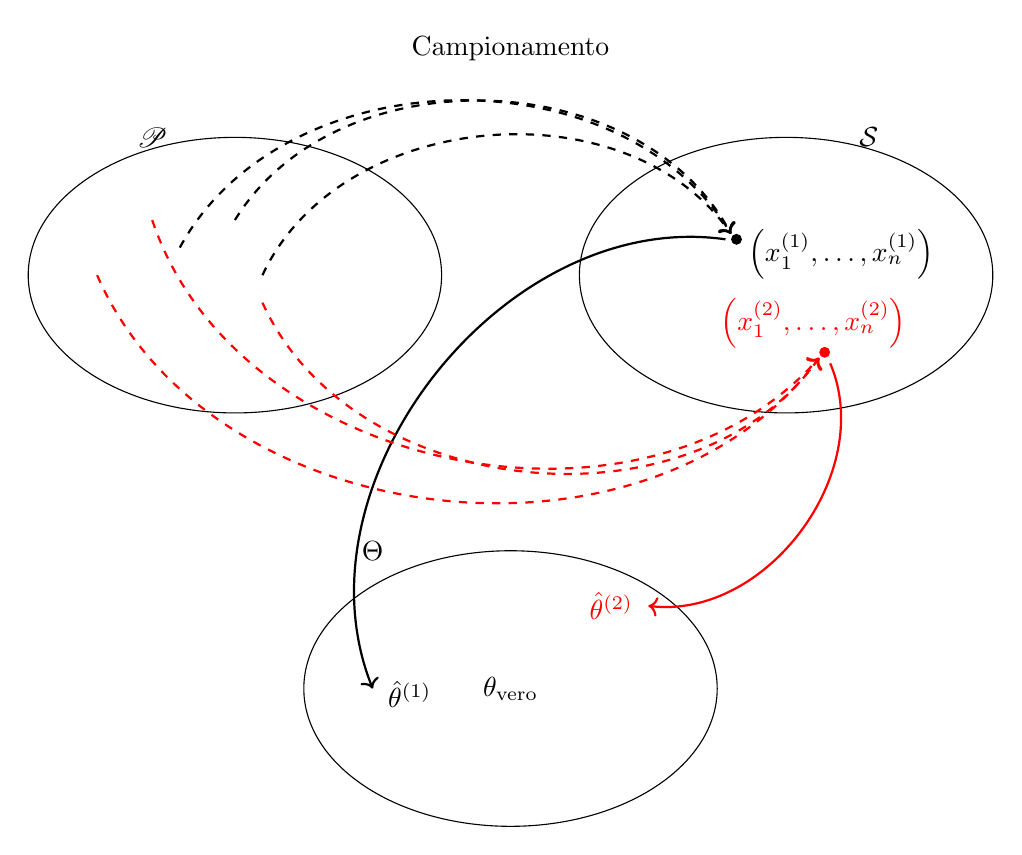
\begin{tikzpicture}[scale=3.5]

% Ellissi
\draw    (-1,1) ellipse (.75 and 0.5);
\draw    (1,1) ellipse (.75 and 0.5);
\draw    (0,-0.5) ellipse (.75 and 0.5);

% Etichette ovali
\node at (-1.3,1.5) {$\mathscr{P}$};
\node at (1.3,1.5) {$\mathcal{S}$};
\node at (-0.5,0) {$\Theta$};
\node at (0,-.5) {$\theta_\text{vero}$};

% Punti osservati
\filldraw (0.82,1.13) circle (.5pt);
\filldraw[fill=red, draw=red] (1.14,0.7+.02) circle (.5pt);

% Etichette osservazioni
\node[align=left, below] at (1.2,1.2) {$\left(x_1^{(1)},\dots,x_n^{(1)}\right)$};
\node[align=left, above, text=red] at (1.1,0.7) {$\left(x_1^{(2)},\dots,x_n^{(2)}\right)$};
\node[align=left, right] at (-0.48,-0.52) {$\hat\theta^{(1)}$};
\node[align=left, left,text=red] at (0.48,-0.2) {$\hat\theta^{(2)}$};
% Frecce nere (campionamento)
  \draw[->, thick, dashed] (-1,1.2) to [bend left=60] (0.8,1.15);
  \draw[->, thick, dashed] (-1.2,1.1) to [bend left=60] (0.8,1.15);
  \draw[->, thick, dashed] (-0.9,1) to [bend left=60] (0.8,1.15);

\draw[->, thick] (0.8-.02,1.13) to [bend left=-60] (-0.5,-0.5);
\draw[->, thick,draw=red] (1.12+.04,0.68) to [bend left=+60] (0.5,-0.2);
% Frecce rosse (secondo campione)
  \draw[->, thick, dashed, draw=red] (-1.5,1) to [bend left=-60] (1.12,0.7);
  \draw[->, thick, dashed, draw=red] (-0.9,0.9) to [bend left=-60] (1.12,0.7);
  \draw[->, thick, dashed, draw=red] (-1.3,1.2) to [bend left=-60] (1.12,0.7);

% Etichetta del processo
\node[below] at (0,1.9) {Campionamento};

\end{tikzpicture}
  
  


\end{document}
